\documentclass[boxes]{homework}

% This is a slightly-more-than-minimal document that uses the homework class.
% See the README at http://git.io/vZWL0 for complete documentation.

\name{傅申 PB20000051}        % Replace (Your Name) with your name.
\term{2022 秋}     % Replace (Current Term) with the current term.
\course{编译原理和技术 B}    % Replace (Course Name) with the course name.
\hwnum{2}          % Replace (Number) with the number of the homework.
\hwname{作业}
\problemname{}
\solutionname{解:}
\problemchap{3}

% Load any other packages you need here.
\usepackage[
    a4paper,
    top = 2.54cm,
    bottom = 2.54cm,
    left = 1.91cm,
    right = 1.91cm,
    includeheadfoot
]{geometry}
\fancyfootoffset{0pt} % make fancyhdr work properly
\usepackage{ctex}
\usepackage{subfigure}

\begin{document}
%%%% Problem 3.1 (a) (c) %%%%
\begin{problem}
考虑文法
\begin{equation}
    \begin{aligned}
        S & \to (L) \mid a  \\
        L & \to L, S \mid S
    \end{aligned}
\end{equation}
\begin{parts}
    \part\label{prob:3.1.a}
    建立句子 $(a, (a, a))$ 和 $(a, ((a, a), (a, a)))$ 的分析树.
    \setcounter{enumi}{2}
    \part\label{prob:3.1.c}
    为 \ref{prob:3.1.a} 的两个句子构造最右推导.
\end{parts}
\end{problem}
\begin{solution}
    \ref{prob:3.1.a} 句子 $(a, (a, a))$ 和 $(a, ((a, a), (a, a)))$ 的分析树如下
    图~\ref{fig:3.1.a} 和图~\ref{fig:3.1.b}.
    \begin{figure}[htbp]
        \centering
        \subfigure[$(a, (a, a))$ 的分析树] {
            \label{fig:3.1.a}
            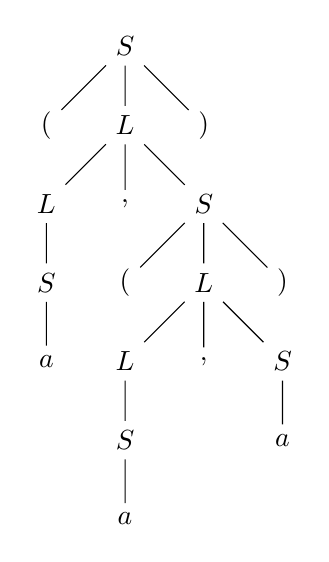
\begin{tikzpicture}[-, level distance=1cm, sibling distance=1cm]
                \node {$S$}
                child {node {(}}
                child {node {$L$}
                        child {node {$L$}
                                child {node {$S$} child {node {$a$}}}
                            }
                        child {node {,}}
                        child {node {$S$}
                                child {node {$($}}
                                child {node {$L$}
                                        child {node {$L$}
                                                child {node {$S$} child {node {$a$}}}
                                            }
                                        child {node {,}}
                                        child {node {$S$} child {node {$a$}}}
                                    }
                                child {node {)}}
                            }
                    }
                child {node {)}};
            \end{tikzpicture}
        }
        \subfigure[$(a, ((a, a), (a, a)))$ 的分析树]{
            \label{fig:3.1.b}
            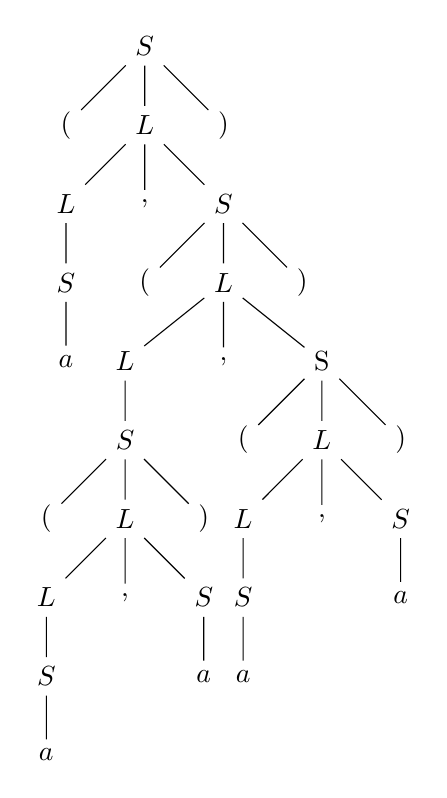
\begin{tikzpicture}[-,
                    level distance=1cm,
                    sibling distance=1cm,
                    level 4/.style={sibling distance=1.25cm},
                    level 5/.style={sibling distance=1cm}]
                \node {$S$}
                child {node {(}}
                child {node {$L$}
                        child {node {$L$}
                                child {node {$S$} child {node {$a$}}}
                            }
                        child {node {,}}
                        child {node {$S$}
                                child {node {(}}
                                child {node {$L$}
                                        child {node {$L$}
                                                child {node {$S$}
                                                        child {node {(}}
                                                        child {node {$L$}
                                                                child {node {$L$}
                                                                        child {node {$S$} child {node {$a$}}}}
                                                                child {node {,}}
                                                                child {node {$S$} child {node {$a$}}}
                                                            }
                                                        child {node {)}}
                                                    }
                                            }
                                        child {node {,}}
                                        child {node {S}
                                                child {node {(}}
                                                child {node {$L$}
                                                        child {node {$L$}
                                                                child {node {$S$} child {node {$a$}}}
                                                            }
                                                        child {node {,}}
                                                        child {node {$S$} child {node {$a$}}}
                                                    }
                                                child {node {)}}
                                            }
                                    }
                                child {node {)}}
                            }
                    }
                child {node {)}}
                ;
            \end{tikzpicture}
        }
        \caption{建立的分析树}
        \label{fig:3.1}
    \end{figure}

    \ref{prob:3.1.c} $(a, (a, a))$ 的最右推导如下
    \begin{equation}
        \begin{aligned}
            S & \Rightarrow (L) \Rightarrow (L, S) \Rightarrow (L, (L))
            \Rightarrow (L, (L, S)) \Rightarrow (L, (L, a)) \Rightarrow
            (L, (S, a)) \Rightarrow (L, (a, a))                         \\
              & \Rightarrow (S, (a, a)) \Rightarrow (a, (a, a))
        \end{aligned}
    \end{equation}
    $(a, ((a, a), (a, a)))$ 的最右推导如下
    \begin{equation}
        \begin{aligned}
            S & \Rightarrow (L) \Rightarrow (L, S) \Rightarrow (L, (L))
            \Rightarrow (L, (L, S)) \Rightarrow (L, (L, (L))) \Rightarrow
            (L, (L, (L, S))) \Rightarrow (L, (L, (L, a)))                 \\
              & \Rightarrow (L, (L, (S, a))) \Rightarrow (L, (L, (a, a)))
            \Rightarrow (L, (S, (a, a))) \Rightarrow (L, ((L), (a, a)))
            \Rightarrow (L, ((L, S), (a, a)))                             \\
              & \Rightarrow (L, ((L, a), (a, a)))  \Rightarrow
            (L, ((S, a), (a, a))) \Rightarrow (L, ((a, a), (a, a))) \Rightarrow
            (S, ((a, a), (a, a)))                                         \\
              & \Rightarrow (a, ((a, a), (a, a)))
        \end{aligned}
    \end{equation}
\end{solution}

%%%% Problem 3.2 (a) %%%%
\begin{problem}
考虑文法
\begin{equation}
    S \to aSbS \mid bSaS \mid \varepsilon
\end{equation}
\begin{parts}
    \part\label{prob:3.2.a}
    为句子 $abab$ 构造两个不同的最左推导, 以此说明该文法是二义的.
\end{parts}
\end{problem}
\begin{solution}
    \ref{prob:3.2.a} 下式~\ref{eq:3.2.1} 和式~\ref{eq:3.2.2} 是句子 $abab$ 的两
    个不同的最左推导.
    \begin{equation}
        \label{eq:3.2.1}
        S \Rightarrow aSbS \Rightarrow abS \Rightarrow abaSbS \Rightarrow ababS
        \Rightarrow abab
    \end{equation}
    \begin{equation}
        \label{eq:3.2.2}
        S \Rightarrow aSbS \Rightarrow abSaSbS \Rightarrow abaSbS \Rightarrow
        ababS \Rightarrow abab
    \end{equation}
\end{solution}

%%%% Problem 3.3 %%%%
\begin{problem}
下面的二义文法描述命题演算公式, 为它写一个等价的非二义文法.
\begin{equation}
    S \to S\ \mathbf{and}\ S \mid S\ \mathbf{or}\ S \mid \mathbf{not}\ S \mid
    \mathbf{true} \mid  \mathbf{false} \mid (S)
\end{equation}
\end{problem}
\begin{solution}
    因为优先级满足 $() > \mathbf{not} > \mathbf{and} > \mathbf{or}$, 且
    \textbf{not} 是单目运算符, 所以构造出非二义文法如下
    \begin{equation}
        \begin{aligned}
            E & \to E\ \mathbf{or}\ T \mid T                               \\
            T & \to T\ \mathbf{and}\ F \mid F                              \\
            F & \to \mathbf{not}\ F \mid \mathbf{true} \mid \mathbf{false}
            \mid (E)
        \end{aligned}
    \end{equation}
\end{solution}
\end{document}
